% !TeX spellcheck = pl_PL
\documentclass[a4paper,twoside]{article}
\usepackage{polski}
\usepackage[utf8]{inputenc}
\usepackage{graphicx}
\usepackage{amsmath}

\usepackage[unicode, bookmarks=true]{hyperref} %do zakładek
\usepackage{tabto} % do tabulacji
\NumTabs{6} % globalne ustawienie wielkosci tabulacji
\usepackage{array}
\usepackage{multirow}
\usepackage{array}
\usepackage{dcolumn}
\usepackage{bigstrut}
\usepackage{color}
\usepackage[usenames,dvipsnames]{xcolor}
\usepackage{svg}
\usepackage{xfrac}
\usepackage{floatrow}
% Table float box with bottom caption, box width adjusted to content
\newfloatcommand{capbtabbox}{table}[][\FBwidth]
\usepackage{blindtext}
\usepackage{enumerate}
\usepackage{wrapfig}


\setlength{\textheight}{24cm}
\setlength{\textwidth}{15.92cm}
\setlength{\footskip}{10mm}
\setlength{\oddsidemargin}{0mm}
\setlength{\evensidemargin}{0mm}
\setlength{\topmargin}{0mm}
\setlength{\headsep}{5mm}

\newcolumntype{M}[1]{>{\centering\arraybackslash}m{#1}}
\newcolumntype{N}{@{}m{0pt}@{}}

\graphicspath{ {./images/} }

% === Reset inkrementacji sekcji przy nowym parcie === %
\usepackage{titlesec}

\makeatletter
\@addtoreset{section}{part}
\makeatother
\titleformat{\part}[display]
{\normalfont\LARGE\bfseries\centering}{}{0pt}{}

\begin{document}
	
	% ==================================================
	% --- 5. TRANSMISJA DANYCH
	% ==================================================
	\section*{Transmisja danych}
	% ================= ZADANIE 5.1 ==================
	\subsection*{Zadanie}
	\subsubsection*{Treść}
	Stacja robocza jest połączona z serwerem z prędkością 11 [Mbps] i stopą błędów BER = $ 7.3 \cdot 10 ^ {-6} $. Oblicz z jaką średnią prędkością mogą być wysyłane informacje z serwera używając wersji standardowej (\emph{plain vanilla}, \emph{Go Back N}) protokołu TCP. Wynegocjowany segment danych to 768 [B] (ramka w łączu 832 [B]), rozmiar okna to 18.5 [KB], a średni czas RTT to 55 [ms].
	\subsubsection*{Odpowiedź}
	\begin{enumerate}
		\item Notacja BER = $ 7.3 \cdot 10 ^ {-6} $ oznacza, że na 1 milion bitów 7.3 z nich są przekłamane. Wyliczamy z nich liczbę przekłamanych bajtów. Dzielimy obie strony przez 7.3, czyli 1 na 136986.3 bitów jest nieprawidłowy. Aby uzyskać bajty, dzielimy oba przez 8, czyli 1 na 17123.3 bajtów jest przekłamany.
		\item Wyliczamy z tego liczbę przekłamanych ramek:
		$$ \cfrac{17123.3\;[B]}{832\;[B]}\approx20.58 $$
		Wybieramy ramkę w łączu, ponieważ interesują nas przesyłane informacje. Wynik oznacza, że 1 z 21 ramek jest przekłamana.
		\item Teraz liczymy liczbę ramek jaka pomieści się w oknie:
		$$ \cfrac{18.5\;[kB]}{768\;[B]}=\cfrac{18\:944\;[B]}{768\;[B]}\approx24.67 $$
		Wybieramy liczbę danych w segmencie, ponieważ interesuje nas to co może pomieścić okno. Z obliczeń wynika, że wielkość okna jest równa 24 ramki + kawałek 25ej, połowa z tego to 12 z groszami. Wynika z tego, że 12 jest granicą, a po niej zaczynami naliczać wg \emph{Congestion Avoidance}.
		\item Możemy przystąpić do rysowania słupków:
		\begin{center}
			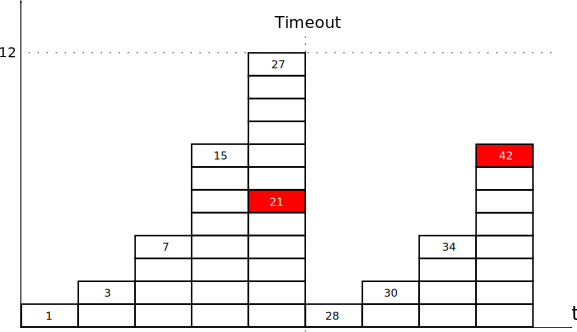
\includegraphics[width=10.0cm]{./images/zadanie16}
		\end{center}
		Liczba ramek rośnie eksponencjalne aż napotka limit w postaci \emph{slow start threshold}u. Nie przekracza go. Gdyby w piątej kolumnie nie wystąpił błąd, liczba ramek w kolejnych rosłaby liniowo. W protokole standardowym, \emph{plain vanilla}, rozmiar okna oraz treshold się nie zmieniają.
		\item Można przystąpić do wyliczenia szybkości. Ponieważ w treści zadania interesuje nas "retransmisja grupowa", obliczamy tylko GNB.
		$$ GBN=\cfrac{(42-8)\cdot832\;[B]}{9\cdot55\;[ms]}\approx470626.26\;[\frac{b}{s}]\approx0.47069\;[Mbps]   $$
		
	\end{enumerate}
	
	
\end{document}